\section{Appendices}

\textcolor{teal}{\subsection{Appendix 1 - Problem Formulation}}

\subsubsection{6-3-5 Method}
\subsubsection*{Hardware \& Mechanics}
\begin{itemize}
    \item use a servo motor for deadbolt control
    \item hall effect sensor to detect if the door is open or closed
    \item implement linear actuator for silent locking
    \item maybe anti-backlash gears to reduce mechanical play
    \item consider designing a modular lock housing with 3D-printed parts
    \item have a backup battery to ensure operation during power outages
\end{itemize}

\subsubsection*{Smartphone Integration}
\begin{itemize}
    \item develop a smartphone app for remote locking/unlocking
    \item push notifications for lock activity (ex: ``Door locked at 3:45 PM'')
    \item have biometric authentication (Face ID or fingerprint)
    \item Use Bluetooth for proximity-based auto-unlock
    \item NFC support for quick unlocking via phone tap
    \item include multi-user access control with time-based permissions
\end{itemize}

\subsubsection*{Security Features}
\begin{itemize}
    \item Implement AES-256 encryption for communication between the lock and phone
    \item maybe two-factor authentication for app access
    \item develop a tamper-detection alarm if the lock is forced
    \item lockdown mode for multiple failed attempts
    \item include a manual override mechanism in case of system failure
    \item utilize rolling codes for Bluetooth pairing to prevent hacking
\end{itemize}

\subsubsection*{Software \& Control}
\begin{itemize}
    \item ESP32 microcontroller for Wi-Fi and Bluetooth control
    \item Develop a closed-loop system to verify if the lock is engaged properly
    \item make a real-time event log accessible via the app
    \item add a scheduling feature for auto-locking at specific times
    \item guest mode with temporary passcodes
    \item Integration with voice assistants like Alexa or Google Assistant
\end{itemize}

\subsubsection*{Advanced Features}
\begin{itemize}
    \item GPS stuff
    \item add geofencing to lock or unlock based on the user's location
    \item integrate with smart home platforms like Home Assistant
    \item use AI-based behavior analysis to suggest locking patterns
    \item add a camera with facial recognition for auto-unlock
    \item enable remote firmware updates
    \item learn database SQL
    \item use solar charging for battery-powered locks
\end{itemize}

% BRAINSTORMING -----------------------------

\subsubsection{Brainstorming}

\subsubsection*{Adam Wu}
\begin{itemize}
    \item As a person who has amnesia, I would like to be able to find my keys anytime so that when I forget where I place them, I can find them.
    \begin{itemize}
        \item Having a "find my" solution with a key.
    \end{itemize}
    \item As a person who loves security, I would like to have the best lock for my house so that lock pickers are not able to pick my lock.
    \begin{itemize}
        \item Making an “authentication” key that resets the key code within a set time, making it harder for hackers to unlock the door.
    \end{itemize}
    \item As a person who is always last-minute out the door, I fear forgetting to lock the door when I close it.
    \begin{itemize}
        \item Auto-locking door when a person closes the door.
    \end{itemize}
    \item As a person who often forgets to bring their keys, I am scared of getting locked out.
    \begin{itemize}
        \item Having a notification from the key to the phone that alerts: “keys are not close by to you.”
    \end{itemize}
    \item As a parent, I am scared of my kids forgetting their keys and locking themselves out of their room.
    \begin{itemize}
        \item Creating a “master key” that only parents/admins can use to unlock specific doors.
    \end{itemize}
    \item Concerned about key battery life.
    \begin{itemize}
        \item Send a notification to the user when the key is on low battery.
    \end{itemize}
\end{itemize}

\subsubsection*{Nathaniel Laurente}
\begin{itemize}
    \item Key has the ability to notify the user when too far away from the user’s phone/body.
    \item Key deactivates/won’t be able to open the door if too far away from the owner.
    \item “Tap to Pay” technology concept.
    \begin{itemize}
        \item Unlocks the door like a credit card tap on a phone.
        \item If too complex, explore alternative ways to unlock the door.
        \item Eliminates the need for a physical key.
        \item Prevents stolen keys from working if the user still has their phone.
    \end{itemize}
    \item Secure deactivation of the key when too far from the user.
    \begin{itemize}
        \item Possible solution: Use the user's phone for deactivation.
    \end{itemize}
    \item One-time password generator between lock and key to ensure only this exact key can enter the house.
    \item Backup way to get into the house if the user forgets/loses their key.
    \begin{itemize}
        \item Pin access code.
        \item App allows for 2FA authentication using a thumbprint and/or Face ID.
    \end{itemize}
    \item Will the battery last long enough for multiple years?
\end{itemize}

\subsubsection*{Neena Nguyen}
\begin{itemize}
    \item Existing smart lock solutions:
    \begin{itemize}
        \item Smart locks for dorm rooms using mobile apps, passcodes, and scanners.
    \end{itemize}
    \item Who will use this lock?
    \begin{itemize}
        \item People with memory issues (elderly, ADHD).
        \item University students in dorm rooms.
        \item Student ID scanner integration.
        \item Parents with small children (child-proof locks).
    \end{itemize}
    \item Features for parental control.
    \begin{itemize}
        \item Locks after a curfew time.
        \item Prevents children from unlocking without parental approval.
        \item Alerts parents when kids come home from school.
    \end{itemize}
    \item What kind of door lock will it be?
    \begin{itemize}
        \item Facial recognition (requires camera and database knowledge).
        \item Logs entry and exit timestamps.
        \item Digital passcode through an app.
        \item Auto-relocking mechanism after failed attempts.
        \item Bluetooth detection for unlocking within a certain range.
        \item Dual authentication (PIN + scan).
        \item Optional security trigger after specific hours.
        \item Alerts when the door is left unlocked for too long.
        \item Auto-locking after prolonged unlocking.
        \item Detection system to check if the key is on the person.
        \item Prevents intruders from entering without a key.
    \end{itemize}
\end{itemize}

\subsubsection*{Jackson Kennedy}
\begin{itemize}
    \item Normal keys can be lock-picked, but digital keys can be secured based on a communication protocol.
    \item Secure authentication methods.
    \begin{itemize}
        \item PIN authentication with 2FA.
        \item Optimal PIN length (e.g., 4-digit PIN has 1,048,576 combinations).
        \item Brute force prevention strategies.
    \end{itemize}
    \item Preventing communication protocol vulnerabilities.
    \begin{itemize}
        \item What protocol should be used? (Bluetooth has vulnerabilities and short range.)
        \item Cloud-based solutions rely on third-party vendor security.
        \item What information needs to be transferred? (Video data, authentication signals?)
    \end{itemize}
    \item Lock activation logic.
    \begin{itemize}
        \item How exactly will the lock know when to unlock? (Sending a 0 or 1 signal based on specific conditions?)
    \end{itemize}
    \item Security and alerting technologies.
    \begin{itemize}
        \item Sensors to detect nearby people.
        \item Hidden camera or biometric verification for identity confirmation.
    \end{itemize}
    \item Scheduling and timed access.
    \begin{itemize}
        \item Physical locks do not have scheduling options.
        \item Implement timed unlocking (e.g., unlock for 15 minutes for a babysitter).
        \item Extra verification to prevent intruders from exploiting schedules.
    \end{itemize}
\end{itemize}
\newpage

% Begin Morphological Charts ----------------------------------

\subsubsection{Morphological Charts}

\begin{figure}[!ht]
    \centering
    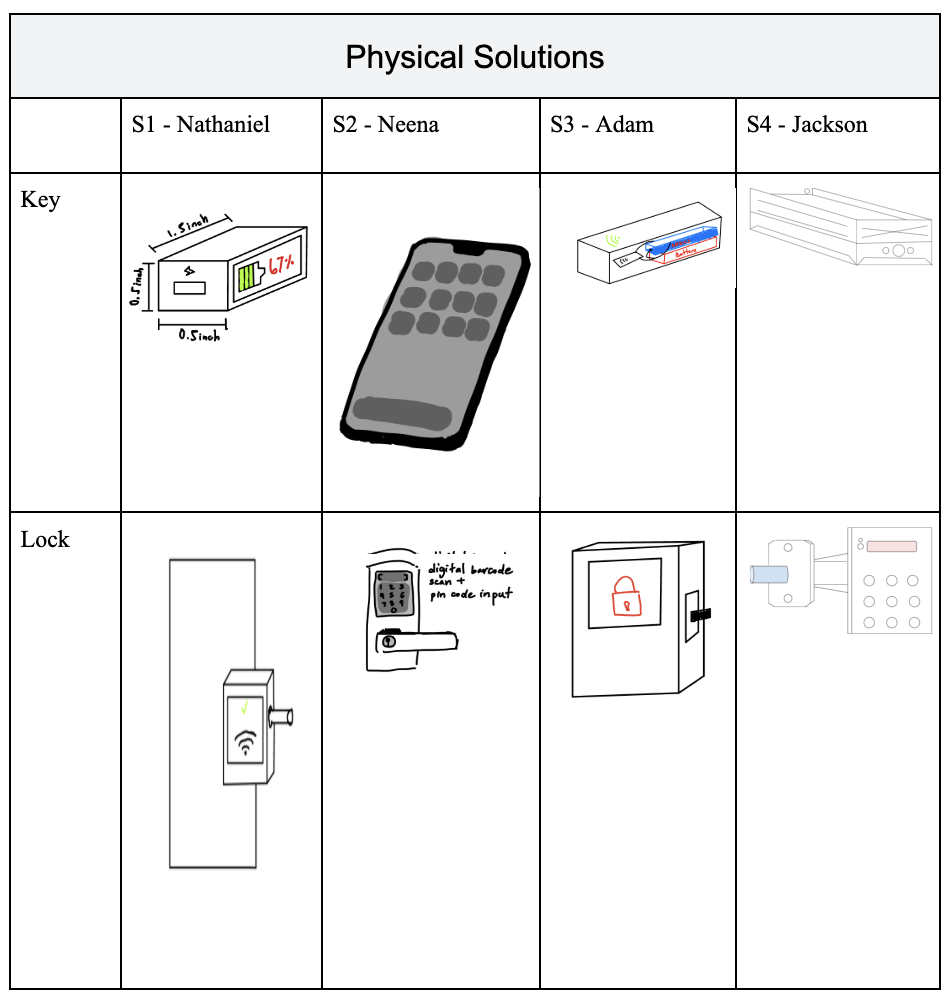
\includegraphics[width=1\linewidth]{./img/p1mm.png}
    \caption{Physical Solution Chart}
    \label{fig:p1mm}
\end{figure}
\newpage
\begin{figure}[!ht]
    \centering
    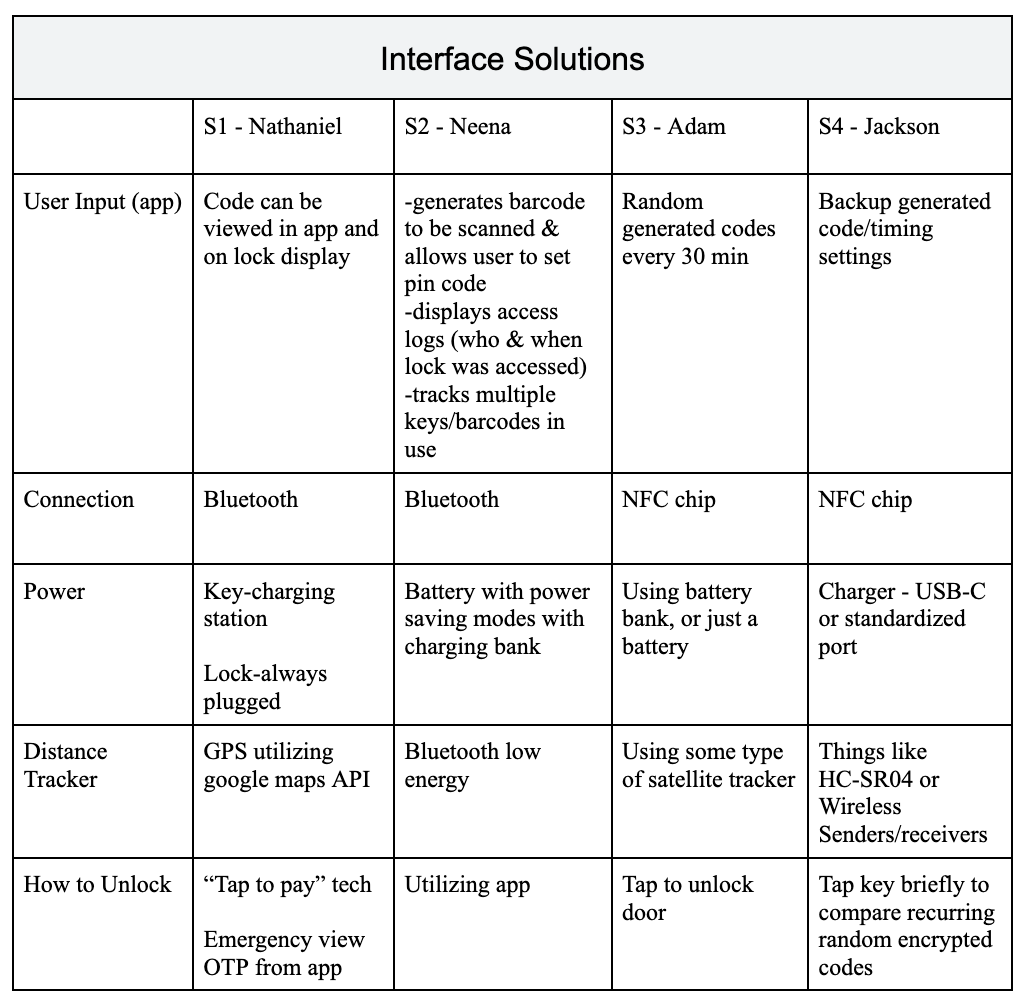
\includegraphics[width=1\linewidth]{./img/p2mm.png}
    \caption{Interface Solutions}
    \label{fig:p2mm}
\end{figure}
\newpage

% Begin Mind Map ---------------------------------------------

\subsubsection{Mind Map}

\begin{figure}[!ht]
    \centering
    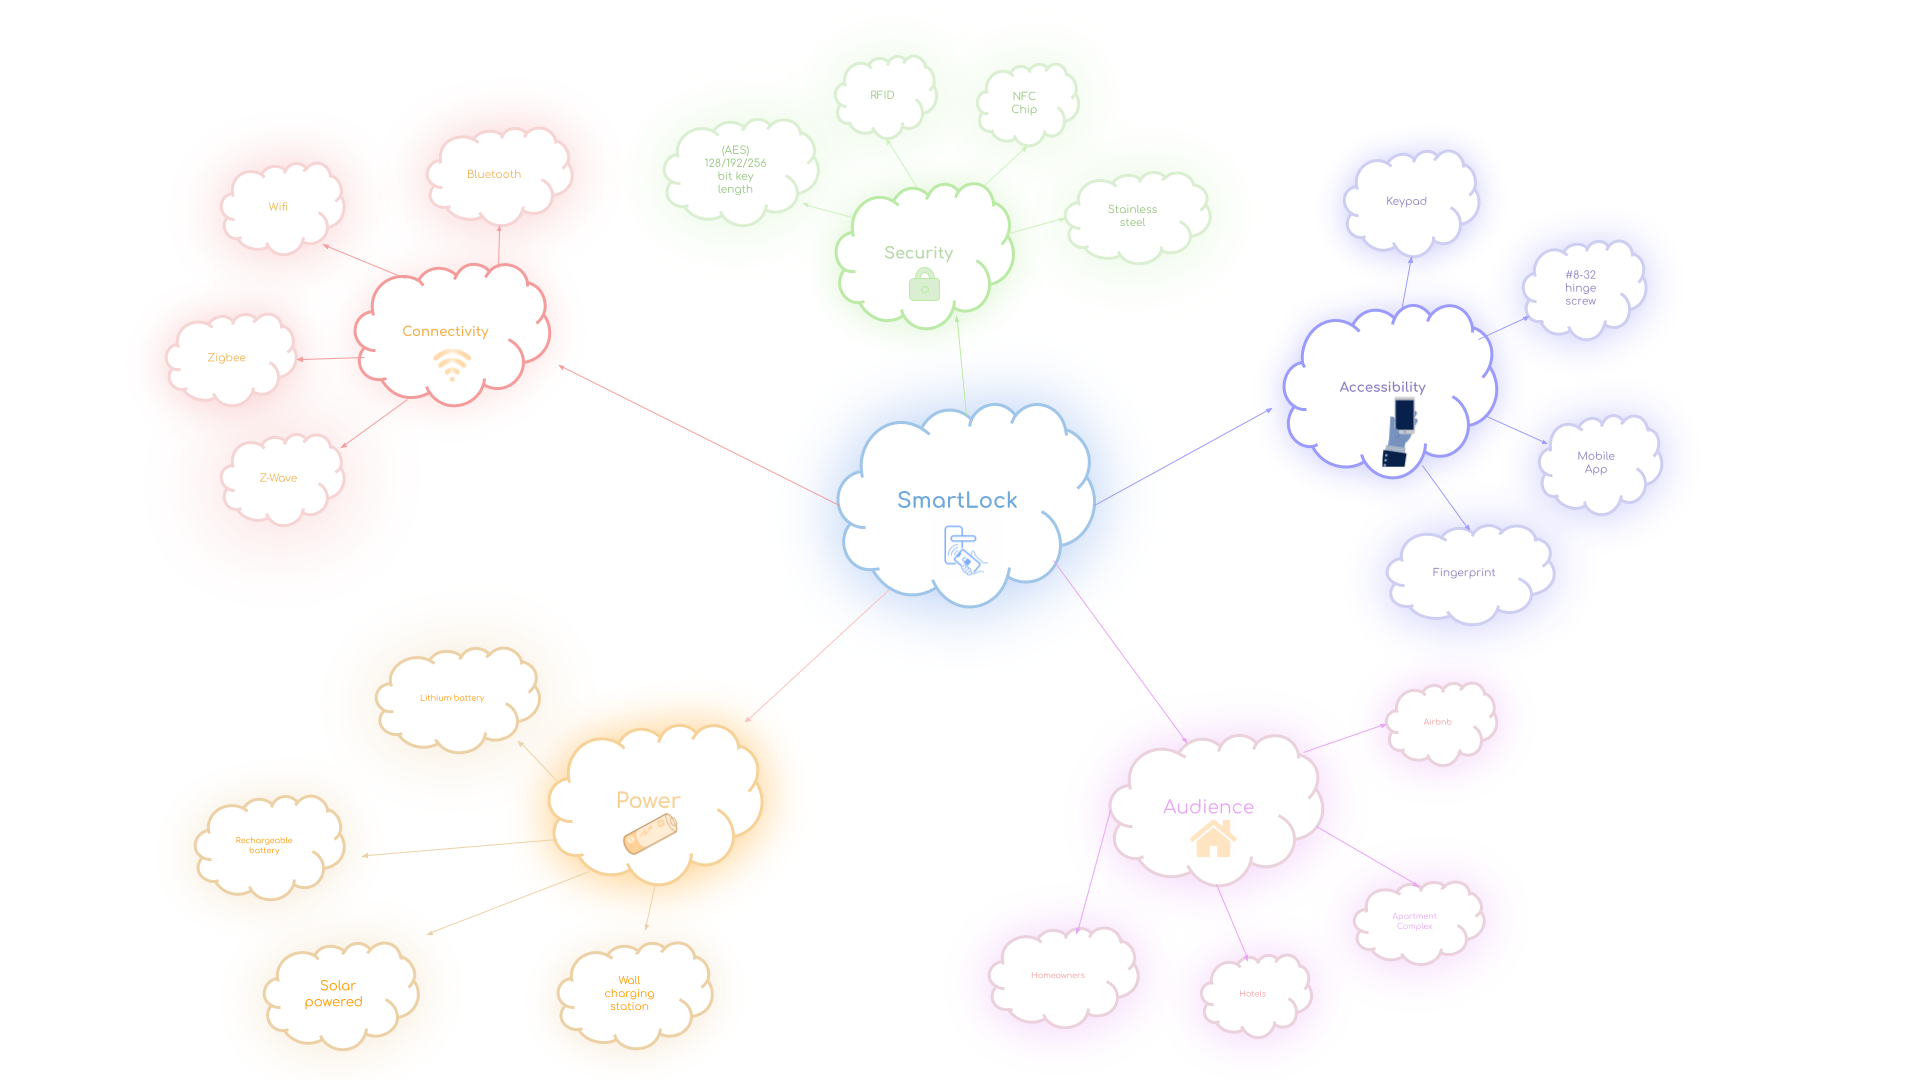
\includegraphics[width=140mm,scale=0.5]{./img/mindmapsmartlock.png}
    \caption{Mind Map}
    \label{fig:mindmapsmartlock}
\end{figure}

\subsubsection{Concept Selection}
\subsubsection*{Weighting Factors}
\begin{tabular}{ll}
    \toprule
    Criteria & Weight (\%) \\
    \midrule
    Security & 40 \\
    Cost & 30 \\
    Power Consumption & 20 \\
    User Convenience & 10 \\
    \textbf{Total} & \textbf{100} \\
    \bottomrule
\end{tabular}

\subsubsection*{Decision Table}
\resizebox{\textwidth}{!}{%
\begin{tabular}{lcccc}
    \toprule
    Criteria & Weight & Design 1 (Basic) & Design 2 (Mid-Range) & Design 3 (Advanced) \\
    \midrule
    Security & 40 & 6 (240) & 8 (320) & 10 (400) \\
    Cost & 30 & 10 (250) & 6 (150) & 3 (75) \\
    Power Consumption & 20 & 6 (90) & 8 (120) & 10 (150) \\
    User Convenience & 10 & 3 (30) & 6 (60) & 9 (90) \\
    \textbf{Total Score} & \textbf{100} & \textbf{680} & \textbf{720} & \textbf{780} \\
    \bottomrule
\end{tabular}%
}

\textbf{Best Design:} Design 3 (Advanced) with 780 points, prioritizing security, cost-efficiency, and power optimization.


\newpage

    \subsection{Appendix 2 - Planning}
    \subsubsection{Gantt Chart}

    \begin{figure}[!ht]
    \centering
    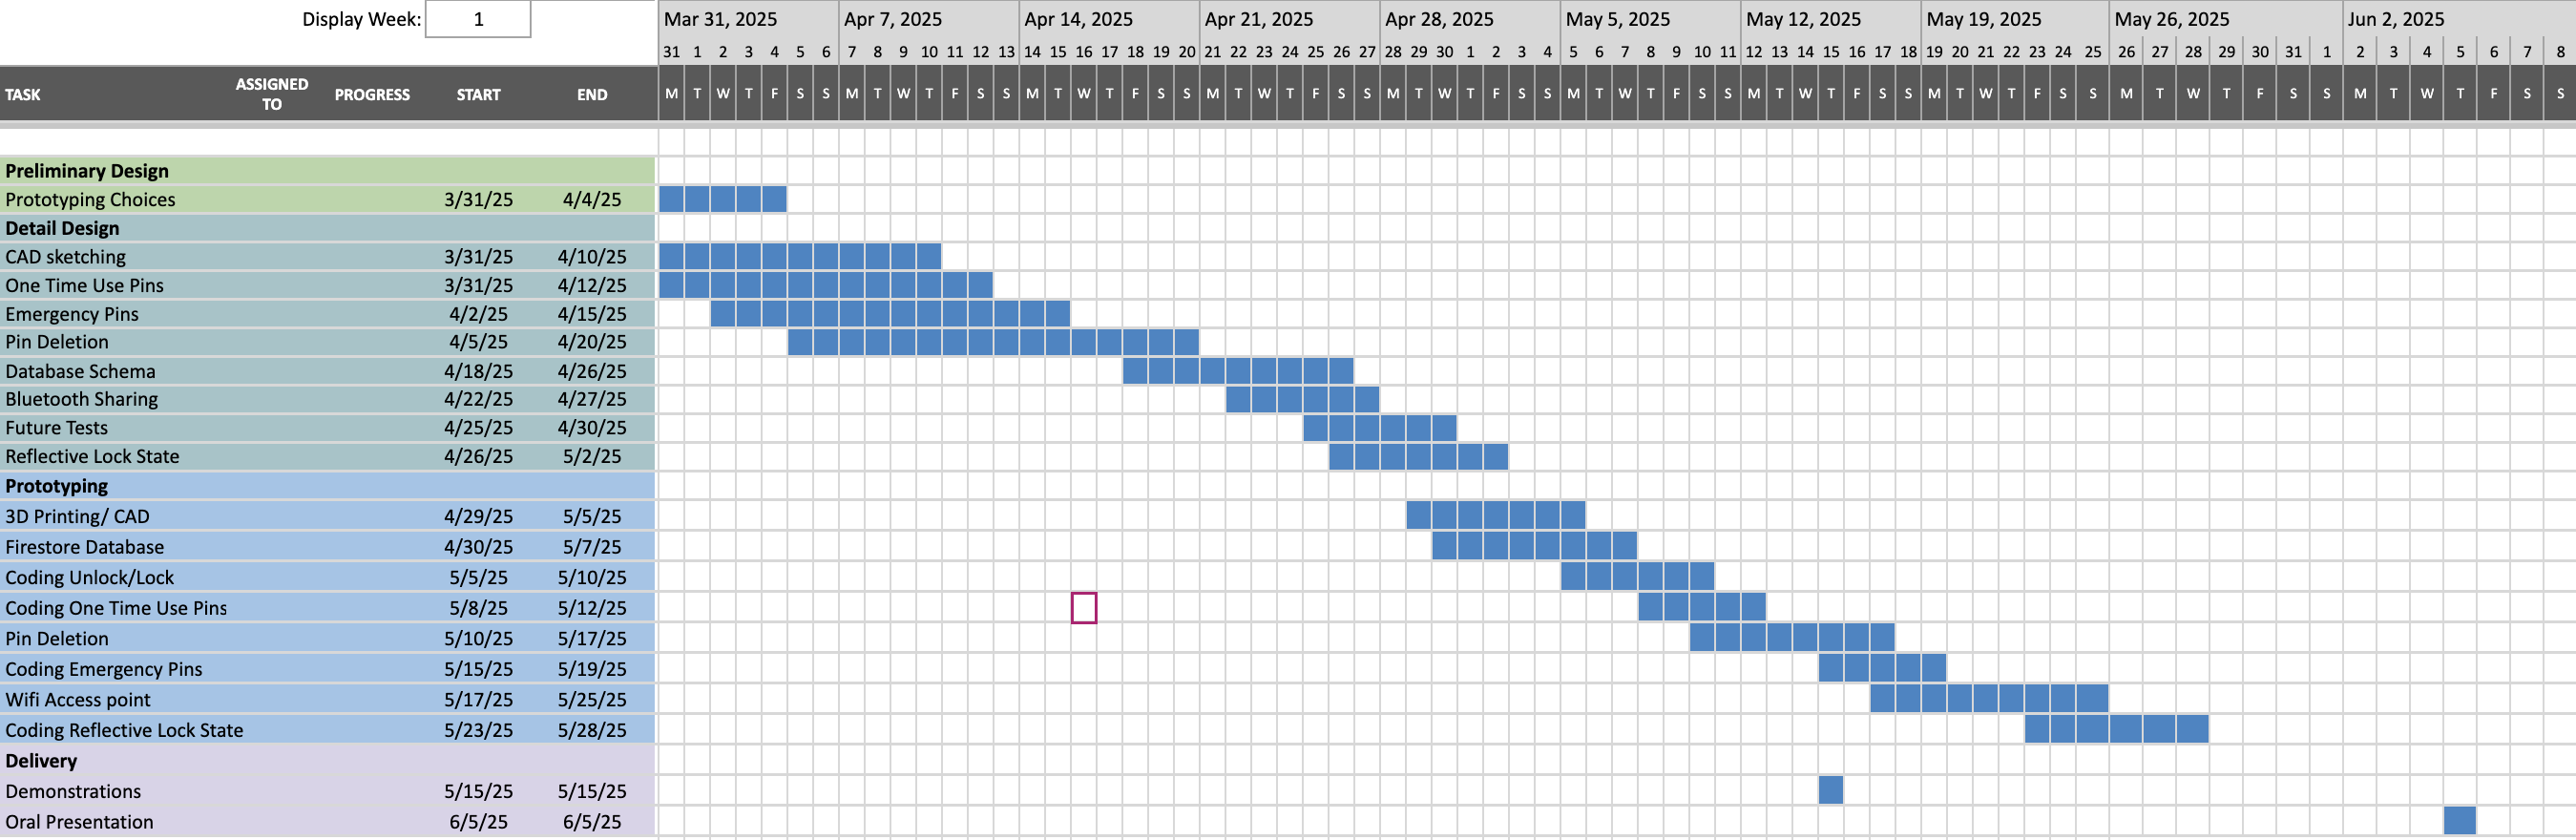
\includegraphics[width=0.80\textwidth]{img/ganttchart.png}
    \caption{Gantt Chart}
    \label{fig:ganttchart}
\end{figure}

\subsubsection{Division of Labor During Prototyping Phase}

Each team member contributed to different aspects of the system based on their strengths: \\

\textbf{Adam} focused on connectivity and user feedback through the hardware. He designed the Wi-Fi configuration process using an access point hosted by the ESP32-C3, allowing users to enter their network credentials during setup. He also implemented visual feedback through LEDs to indicate key system events like Wi-Fi disconnection and keypad input, which improved user interaction and made the system more transparent and intuitive. In addition to handling the microcontroller logic for reading and writing PIN codes, he also worked on sending acknowledgment signals to the database to reflect lock status. Adam read extensive documentation and shared his findings with the team, helping everyone better understand and use specific library functions needed for the embedded system. \\

\textbf{Jackson} handled mobile app development and the various components and package dependencies within it. Using Swift and Xcode, he built the app to support account creation, user authentication, locking and unlocking functions, and the generation of one time and emergency PINs. He implemented additional layers of security, including key protections for the emergency pins, and ensured the app could successfully interact with the Firestore database. This included writing data based on user actions as well as receiving values from the microcontroller. He focused on correctly storing, updating, and modifying values in response to user interactions, and handled database reads that reflected lock activity such as acknowledgement signals confirming a successful unlock. He made sure those values were then displayed in the app’s UI to keep the user informed of the lock’s state in real time. \\

\textbf{Nathaniel} worked on the embedded systems logic that connected keypad input to the solenoid lock’s behavior. He ensured the ESP32-C3 could correctly interpret keypad entries from the keypad and respond appropriately based on the type of PIN entered. He also developed the core functionality behind the one time PINs and emergency PINs, ensuring that they operated securely and reliably within different usage scenarios. In addition to his implementation work, Nathaniel designed and led many of the functional testing cases that helped us validate how the system responded to various edge cases, user actions, and failure conditions. He also contributed to the two-way acknowledgement system between the ESP32-C3 and Firestore, confirming that PIN entries were recognized and matched against those generated by the mobile application. \\

\textbf{Neena} focused on the physical and backend infrastructure of the project. Neena led the CAD design of the smart lock enclosure using Fusion 360, despite having no prior experience with CAD tools. Through tutorials, peer examples, and trial and error, she taught herself how to design for 3D printing and gradually refined the model over several iterations. Her final design featured a clean, minimal container with both top and bottom openings for easier assembly, accounted for hardware fit issues like oversized breadboards and solenoid lock dimensions, and included a small window to make the LED indicators visible from outside. Neena also took charge of defining the Firestore database schema. The system initially supported a basic one-to-many relationship where one user could access multiple locks, but Neena recognized that this would be too limiting for real world use cases. She advocated for and designed a more flexible many-to-many model, allowing multiple users to share access to multiple locks. This included structuring user and lock collections separately, and introducing a join collection to manage shared permissions and access levels. While the full implementation of this schema wasn’t completed due to time constraints, her planning laid a foundation for scaling the access control logic in future versions of the product. \\

All members contributed to system integration, documentation, poster/presentation design, and final testing.

\subsubsection{Collaboration}

We worked closely as a team throughout the entire project, meeting regularly both in person and over Discord. In person sessions were especially helpful when it came to debugging, assembling the prototype, and running tests, while Discord helped us stay connected between meetings and keep progress moving asynchronously. \\

We used GitHub to manage version control, pushing and reviewing code through pull requests and keeping our work organized across different components. While we each focused on our own areas like app development, CAD, or firmware, we were always checking in with each other, helping troubleshoot bugs, and making decisions together when things didn’t go as expected. \\

We also utilized the Arduino IDE for the ESP32-C3 firmware, which allowed us to share code snippets and collaborate on the microcontroller logic. This was particularly useful for integrating the keypad input with the solenoid lock and ensuring that the Firestore database updates were correctly reflected in the mobile app. We used the Arduino IDE because it contained all the libraries needed for firestore and ESP32-C3 development. \\

As we got closer to the deadline, collaboration became even more hands on. We met frequently to run hardware tests, make final tweaks to the CAD design, rehearse the demo, and wrap up our documentation and poster. Even though we had separate roles, we shared a strong sense of team ownership, which helped keep the project on track and made the experience feel really rewarding. \\

\newpage
\begin{samepage}
    \section{Manufactured Product Testing}
    \subsection{Common Scenarios (Tests 1–10)}
% ---------------------------- Test 1 --------------------------------
    \subsection*{1. Valid PIN Entry Test}
    \subparagraph{Test Goals and Purpose}
    \begin{itemize}
        \item Verify that a recognized 4-digit PIN unlocks the door without unnecessary delay.
        \item Check that the system logs this event as a successful access in Firestore.
    \end{itemize}
    \subparagraph{How We Test It}
    \begin{enumerate}
        \item Select a PIN known to be valid from the internal list.
        \item Enter the PIN once on the keypad.
        \item Observe the system's response, checking for physical bolt movement and UI changes on the mobile application.
        \item Look for updates to the (\texttt{LOCK\_STATE}) value in Firestore.
    \end{enumerate}
    
    \textbf{Expectations of Test}
    \begin{center}
    \begin{tabular}{|c|p{10cm}|}
      \hline
      \textbf{Result} & \textbf{Conditions} \\
      \hline
      PASS & Bolt retracts within \textless{}0.5\,s; \texttt{LOCK\_STATE}=1; Firestore log entry \emph{success}. \\
      \hline
      FAIL & Any deviation from the above timing, state, or logging behaviour. \\
      \hline
    \end{tabular}
    \end{center}
\end{samepage}


% ---------------------------- Test 2 --------------------------------
\newpage
\subsection*{2. Invalid PIN Lockout Test}
\subparagraph{Test Goals and Purpose}
\begin{itemize}
    \item Ensure the system prevents further PIN attempts after multiple consecutive failures.
    \item Lock should be shut down for a short expiration period.
    \item Confirm some form of lockout indication is presented, such as a light or warning beep.
    \item Owner's phoone should receive an alert about the failed attempts.
\end{itemize}
\subparagraph{How We Test It}
\begin{itemize}
    \item Enter three clearly incorrect PINs in under 30 seconds.
    \item Observe for a visible or audible signal.
    \item Confirm that \texttt{LOCKOUT\_COUNT} has risen and \texttt{LOCK\_STATE} is still 0 (locked).
\end{itemize}
\subparagraph{Expectations of Test}
\begin{center}
\begin{tabular}{|c|p{10cm}|}
  \hline
  \textbf{Result} & \textbf{Conditions} \\
  \hline
  \textbf{PASS} &
    \begin{minipage}[t]{\linewidth}
    \begin{itemize}
      \item Keypad flashes red and/or beeps immediately after the \textbf{third} wrong entry.
      \item No further PINs are accepted for the lockout period (default: 60 s).
      \item Mobile app log shows “3 invalid PIN attempts – lock is temporarily disabled” within 5 s.
      \item Firestore records \texttt{LOCKOUT\_COUNT = 3} and \texttt{LOCK\_STATE = 0}.\\
    \end{itemize}
    \end{minipage} \\ 
  \hline
  \textbf{FAIL} & Any one of the PASS conditions is missing or incorrect. \\ 
  \hline
\end{tabular}
\end{center}
\vspace{0.5em}

\noindent\textbf{Reset after the test:}  
Either wait for the lockout timer to expire or enter an admin PIN to clear the lockout so the next test starts from a clean state.\\


% ---------------------------- Test 3 --------------------------------
\newpage
\begin{samepage}
    \subsection*{3. Emergency PIN Test}
    \subparagraph{Test Goals and Purpose}
    

\subsection*{4. OTP Entry Test}
\subparagraph{Test Goals and Purpose}
\begin{itemize}
    \item Confirm that an app-generated one-time password (OTP) grants access as expected.
    \item Ensure the OTP mechanism is time-bound and secure against reuse.
\end{itemize}
\subparagraph{How We Test It}
\begin{itemize}
    \item Request a 5-minute valid OTP from the app.
    \item Enter the OTP using the keypad.
    \item Monitor the system and database for changes.
\end{itemize}
\subparagraph{Expectations of Test}
\begin{itemize}
    \item Firestore captures the OTP with a clear expiry time.
    \item Valid OTPs allow immediate unlock.
    \item Expired or incorrect OTPs are properly rejected with no unlock attempt.
\end{itemize}

\subsection*{5. OTP Expiry Test}
\subparagraph{Test Goals and Purpose}
\begin{itemize}
    \item Ensure expired OTPs don’t grant access, even if they were once valid.
    \item Confirm that users are informed clearly when an OTP is no longer usable.
\end{itemize}
\subparagraph{How We Test It}
\begin{itemize}
    \item Generate an OTP and wait for the full 5-minute window to pass.
    \item Attempt to use the expired code via the keypad.
\end{itemize}
\subparagraph{Expectations of Test}
\begin{itemize}
    \item Lock remains unchanged and secure—no movement or unlock occurs.
    \item Firestore logs the expired OTP attempt explicitly.
    \item App and/or interface display an "OTP expired" notification.
\end{itemize}

\subsection*{6. Rapid Wrong PIN Alarm Test}
\subparagraph{Test Goals and Purpose}
\begin{itemize}
    \item Ensure multiple fast wrong PIN entries trigger audible alarm.
    \item Verify lock does not unlock after wrong entries.
    \item Check alarm stops after timeout or correct PIN.
\end{itemize}
\subparagraph{How We Test It}
\begin{itemize}
    \item Enter 5 wrong PINs within 10s.
    \item Observe alarm sound and LOCK\_STATE remains 0.
    \item Attempt correct PIN after alarm to confirm reset.
\end{itemize}
\subparagraph{Expectations of Test}
\begin{itemize}
    \item Alarm beeps continuously for spec duration (e.g., 30s).
    \item Bolt remains locked (LOCK\_STATE = 0).
    \item Firestore logs each failed attempt and alarm event.
    \item Correct PIN after alarm silences alarm and unlocks door.
\end{itemize}

\subsection*{7. Concurrent Unlock Command Test}
\subparagraph{Test Goals and Purpose}
\begin{itemize}
    \item Verify two family phones sending unlock at once doesn't confuse the system.
    \item Ensure only one actuation happens.
    \item Confirm both requests are logged.
\end{itemize}
\subparagraph{How We Test It}
\begin{itemize}
    \item From two phones, send unlock API calls within 100 ms.
    \item Watch bolt movement and LOCK\_STATE.
    \item Check Firestore for two event entries.
\end{itemize}
\subparagraph{Expectations of Test}
\begin{itemize}
    \item Bolt retracts only once.
    \item LOCK\_STATE = 1 after first command.
    \item Both commands logged with timestamps.
    \item No errors or retries triggered.
\end{itemize}

\subsection*{8. Offline Fallback PIN Test}
\subparagraph{Test Goals and Purpose}
\begin{itemize}
    \item Ensure local PIN entry still works if Wi-Fi drops.
    \item Verify lock uses cached PIN list.
    \item Confirm Firestore syncs later.
\end{itemize}
\subparagraph{How We Test It}
\begin{itemize}
    \item Disable Wi-Fi on ESP32, enter valid PIN.
    \item Observe bolt movement and local log.
    \item Re-enable Wi-Fi and check Firestore sync.
\end{itemize}
\subparagraph{Expectations of Test}
\begin{itemize}
    \item Door unlocks locally (LOCK\_STATE = 1 locally).
    \item Event cached and later pushed to Firestore.
    \item No user-perceived delay in unlocking.
    \item Sync event marked with “offline” flag.
\end{itemize}

\subsection*{9. Low-Battery Notification Test}
\subparagraph{Test Goals and Purpose}
\begin{itemize}
    \item Check notification when battery falls below 10 %.
    \item Ensure unlock still works at low battery.
    \item Verify UI warning persists until charge.
\end{itemize}
\subparagraph{How We Test It}
\begin{itemize}
    \item Drain battery to 9 %.
    \item Press unlock PIN and observe behavior.
    \item Check mobile app for low-battery alert.
\end{itemize}
\subparagraph{Expectations of Test}
\begin{itemize}
    \item Door still unlocks (LOCK\_STATE = 1).
    \item App shows persistent “Low Battery” message.
    \item Firestore logs battery level event.
    \item Warning clears only when battery > 20 %.
\end{itemize}

\subsection*{10. Battery Fully Drained Test}
\subparagraph{Test Goals and Purpose}
\begin{itemize}
    \item Verify lock fails to actuate when battery is dead.
    \item Ensure system logs failure and alerts user.
    \item Confirm physical key still works.
\end{itemize}
\subparagraph{How We Test It}
\begin{itemize}
    \item Let battery drop to 0\%.
    \item Enter valid PIN and observe no bolt movement.
    \item Try physical key override.
\end{itemize}
\subparagraph{Expectations of Test}
\begin{itemize}
    \item Bolt does not move on electronic command.
    \item Firestore logs “Battery Depleted” error.
    \item Physical key unlocks door.
    \item App advises “Replace Battery” notification.
\end{itemize}


\subsection*{11. Battery Fully Drained Test}
\subparagraph{Test Goals and Purpose}
\begin{itemize}
    \item Verify lock fails to actuate when battery is dead.
    \item Ensure system logs failure and alerts user.
    \item Confirm physical key still works.
\end{itemize}
\subparagraph{How We Test It}
\begin{itemize}
    \item Let battery drop to 0 \%.
    \item Enter valid PIN and observe no bolt movement.
    \item Try physical key override.
\end{itemize}
\subparagraph{Expectations of Test}
\begin{itemize}
    \item Bolt does not move on electronic command.
    \item Firestore logs “Battery Depleted” error.
    \item Physical key unlocks door.
    \item App advises “Replace Battery” notification.
\end{itemize}

























\newpage
\subsection{Less Common Scenarios (Tests 31–40)}

\subsection*{31. Multi-factor Auth Proximity Test}
\subparagraph{Test Goals and Purpose}
\begin{itemize}
    \item Confirm the system requires both a valid PIN and Bluetooth proximity to unlock.
    \item Observe behavior if Bluetooth disconnects mid-process.
\end{itemize}
\subparagraph{How We Test It}
\begin{itemize}
    \item Start PIN entry and slowly move the paired phone out of Bluetooth range.
    \item Review logs to see how the system treats incomplete multi-factor input.
\end{itemize}
\subparagraph{Expectations of Test}
\begin{itemize}
    \item Door only unlocks when both factors are simultaneously validated.
    \item Firestore logs clearly show whether it was the PIN or BLE that failed.
\end{itemize}

\subsection*{32. Time-zone Mismatch Test}
\subparagraph{Test Goals and Purpose}
\begin{itemize}
    \item Ensure that timing-sensitive operations work properly despite device time mismatches.
    \item Verify that scheduled actions and OTPs remain aligned regardless of local time zones.
\end{itemize}
\subparagraph{How We Test It}
\begin{itemize}
    \item Set the phone to Pacific Time and the lock to Coordinated Universal Time.
    \item Generate and use an OTP, and observe if the mismatch causes issues.
\end{itemize}
\subparagraph{Expectations of Test}
\begin{itemize}
    \item OTPs still work during their intended validity window.
    \item Scheduled events (e.g., auto-lock) trigger based on synchronized absolute times.
\end{itemize}

\subsection*{33. DST Transition Auto-lock Test}
\subparagraph{Test Goals and Purpose}
\begin{itemize}
    \item Confirm that daylight saving time transitions don't disrupt automated locking.
\end{itemize}
\subparagraph{How We Test It}
\begin{itemize}
    \item Schedule an auto-lock event for 2:00 AM on the day of the DST shift.
    \item Observe actual lock behavior before, during, and after the transition.
\end{itemize}
\subparagraph{Expectations of Test}
\begin{itemize}
    \item Only one auto-lock event occurs, even with the clock shift.
    \item No skipped or duplicated scheduling happens.
\end{itemize}

\subsection*{34. Admin vs. Guest Role Change Test}
\subparagraph{Test Goals and Purpose}
\begin{itemize}
    \item Validate that role-based access control takes effect immediately after role changes.
\end{itemize}
\subparagraph{How We Test It}
\begin{itemize}
    \item Change a user's role (e.g., from guest to admin) directly in Firestore.
    \item Attempt access under both roles shortly after the change.
\end{itemize}
\subparagraph{Expectations of Test}
\begin{itemize}
    \item The new role is honored without requiring system restart or delay.
    \item Access permissions align with the updated role instantly.
\end{itemize}

\subsection*{35. BLE Range Boundary Test}
\subparagraph{Test Goals and Purpose}
\begin{itemize}
    \item Determine the Bluetooth unlocking behavior at different physical distances.
\end{itemize}
\subparagraph{How We Test It}
\begin{itemize}
    \item Gradually move the phone away from the lock in 0.5-meter steps, from 1 m up to 6 m.
    \item Test unlocking at each position and note the results.
\end{itemize}
\subparagraph{Expectations of Test}
\begin{itemize}
    \item Unlocks reliably at closer distances.
    \item Fails gracefully beyond Bluetooth’s effective range.
\end{itemize}










































\newpage
\subsection{Rare Scenarios (Tests 61–65)}

\subsection*{61. Cosmic Ray Bit-Flip Test}
\subparagraph{Test Goals and Purpose}
\begin{itemize}
    \item Evaluate the system’s resilience to random memory errors, such as those caused by cosmic rays.
\end{itemize}
\subparagraph{How We Test It}
\begin{itemize}
    \item Use a simulator to inject random bit flips into RAM and flash every 10 seconds.
    \item Observe system behavior over an extended period.
\end{itemize}
\subparagraph{Expectations of Test}
\begin{itemize}
    \item System detects and handles bit errors—either by correcting or isolating them.
    \item No persistent crashes or loss of functionality.
\end{itemize}

\subsection*{62. Lightning Surge Test}
\subparagraph{Test Goals and Purpose}
\begin{itemize}
    \item Assess whether the hardware can tolerate sudden electrical surges.
\end{itemize}
\subparagraph{How We Test It}
\begin{itemize}
    \item Apply a 1-kV spike to the 12V input for a 1 microsecond duration using a surge generator.
\end{itemize}
\subparagraph{Expectations of Test}
\begin{itemize}
    \item No hardware is permanently damaged.
    \item System recovers and operates normally after the surge event.
\end{itemize}

\subsection*{63. Seismic Vibration Test}
\subparagraph{Test Goals and Purpose}
\begin{itemize}
    \item Verify the lock’s mechanical and electronic components withstand prolonged shaking.
\end{itemize}
\subparagraph{How We Test It}
\begin{itemize}
    \item Subject the device to a vibration range of 5–50 Hz at 0.5 g for 10 minutes.
    \item Check for loosening, noise, or malfunction.
\end{itemize}
\subparagraph{Expectations of Test}
\begin{itemize}
    \item All parts remain in place and fully operational.
    \item Sensors continue to function accurately post-test.
\end{itemize}

\subsection*{64. Extreme Cold Operation Test}
\subparagraph{Test Goals and Purpose}
\begin{itemize}
    \item Confirm functionality in severe cold conditions down to -40 °C.
\end{itemize}
\subparagraph{How We Test It}
\begin{itemize}
    \item Place the lock in a chamber set to -40 °C for 2 hours.
    \item Perform 10 complete lock/unlock cycles.
\end{itemize}
\subparagraph{Expectations of Test}
\begin{itemize}
    \item Mechanism operates without freezing or delay.
    \item No cracking or material degradation.
    \item Battery and electronics remain reliable.
\end{itemize}

\subsection*{65. Extreme Heat Operation Test}
\subparagraph{Test Goals and Purpose}
\begin{itemize}
    \item Test device reliability when exposed to 85 °C for extended periods.
\end{itemize}
\subparagraph{How We Test It}
\begin{itemize}
    \item Place the lock in a heat chamber at 85 °C.
    \item Execute a lock/unlock cycle every 5 minutes over 2 hours.
\end{itemize}
\subparagraph{Expectations of Test}
\begin{itemize}
    \item No thermal shutdown or malfunctions.
    \item MCU and storage remain intact and responsive.
\end{itemize}


\newpage
\subsection{Appendix 4 - Review}
    \subsubsection*{Nathaniel Laurente}
    Throughout the quarter, designing our smart lock proved very difficult when delving into the details of each component. I believe starting on the prototype early went very well for us since we were able to do our demonstration with all the features we wanted to prove through it. Researching how to design our manufactured product was difficult. We didn’t realize how hard it would be to find and design parts for an actual industry grade product, nor really delve into many different edge cases to see if these parts fit our needs to pass certain tests. We managed to find all the right parts, database, tools, manufacturing processes, and software needed to produce what we thought could be a potentially marketable product. As a team, it was an interesting experience to set up tasks on our GitHub, and coordinate times for meeting up or completing certain aspects of the final design and prototype.

    \subsubsection*{Adam Wu}
    Over the course of this project, I learned a lot-especially about teamwork and how to effectively use GitHub for collaboration. I enjoyed the process of problem-solving and working through challenges as a team. The struggle itself was a valuable part of the experience. One of the things that went well was how we supported each other and made steady progress, especially when we were able to meet in person. However one of the biggest challenges we faced was coordinating our schedules to find time to work together physically. We found that our most productive and collaborative moments happened when we were all in the same space, so scheduling conflicts often slowed down our momentum. Despite that, I’m happy with what we accomplished being the smallest team and how much I’ve grown from the experience.

    \subsubsection*{Jackson Kennedy}
    For the duration of this class, I found myself running into problems along the way both programmatically as well as problems with finding times to meet as a group with conflicting schedules and life events. Regardless, we were able to power through these problems and fix code, as well as find common times that when we all were together, proved monumental in progressing the overall project. If we were to do this class over, I think that finding and enforcing a more common schedule where we can all meet in person would be ideal because some of the best work happened when we were all present. One un-avoidable thing was having a changing group size and project path but I believe we handled the change well and were able to deliver on the product scope which made the class very rewarding.

    \subsubsection*{Neena Nguyen}
    One of the most rewarding parts of this project was getting to work closely with my team. We regularly met in person and on Discord to troubleshoot issues, share updates, and figure things out together. Even when things got difficult, especially when deadlines were tight, I enjoyed problem-solving as a unit, not just individually. I also really enjoyed designing the posters and presentation materials for our group. The most rewarding part of this experience was seeing how our ideas slowly turned into something real. We started with a mess of wires and components on a breadboard, and by the end, we had a functioning smart lock prototype with a physical enclosure. Even though there were major technical challenges for me and I was pushed to learn a lot, what stood out most was how much we grew as a team throughout the process. We each had our own roles, but we also made space for each other to give input and ask for help. I felt like I had ownership over specific parts of the project, but never felt like I was working in isolation. If I were to do this again, I’d ask for more guidance early on in the areas I was less familiar with. I’d also try to plan ahead more for the database structure. But overall, I’m proud of how we communicated, adapted, and built something meaningful together.


